\documentclass[manual-fr.tex]{subfiles}
\begin{document}

Dans le but de simplifier les traitements, SEM ne permet pas de modifier le contenu des fichiers via l'interface ou de modifier le jeu d'étiquettes. Ainsi, pour annoter un document il faut :
\begin{itemize}
    \item le charger depuis un fichier;
    \item charger le jeu d'étiquettes depuis un fichier;
\end{itemize}

~

SEM génère des raccourcis clavier depuis le jeu d'étiquettes qui sera chargé. Un fichier contenant un jeu d'étiquettes suit un format "une étiquette par ligne" comme l'exemple suivant :

\begin{lstlisting}[frame=single]
etiquette1

# un commentaire
etiquette2.sous-etiquette1
etiquette2.sous-etiquette2 # un autre commentaire

etiquette3
\end{lstlisting}

SEM gère les étiquettes hiérarchiques et considère le caractère "." comme le séparateur de niveaux entre étiquettes. Les lignes vides sont ignorées et le caractère "\#" permet d'écrire des commentaires qui seront ignorés. Dans notre cas, nous souhaitons gérer les types \emph{logiciel} et \emph{personne}. Le fichier aura alors le contenu suivant :

\begin{lstlisting}[frame=single]
logiciel
personne
\end{lstlisting}

Les figures \ref{fig:annotation_sem-02} et \ref{fig:annotation_sem-03} illustrent comment charger un fichier et un jeu d'étiquettes.

\begin{figure}[ht!]
    \begin{center}
    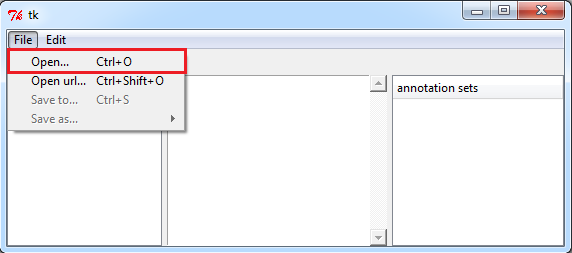
\includegraphics[scale=0.5]{fr/images/annotation_sem-02.png}
    \end{center}
    \caption{Encadré en rouge : l'élément du menu pour charger un fichier.}
    \label{fig:annotation_sem-02}
\end{figure}



\begin{figure}[ht!]
    \begin{center}
    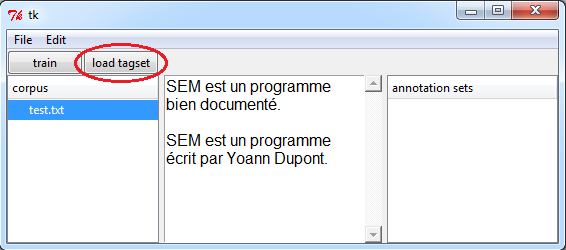
\includegraphics[scale=0.5]{fr/images/annotation_sem-03.png}
    \end{center}
    \caption{Entouré en rouge : le bouton pour charger un jeu d'étiquettes.}
    \label{fig:annotation_sem-03}
\end{figure}


Les figures \ref{fig:annotation_sem-04}, \ref{fig:annotation_sem-05} et \ref{fig:annotation_sem-06} illustrent comment annoter manuellement un corpus puis réentraîner un modèle utilisable par SEM sur ce corpus.


\begin{figure}[ht!]
    \begin{center}
    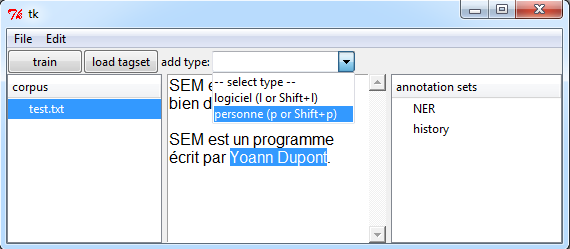
\includegraphics[scale=0.5]{fr/images/annotation_sem-04.png}
    \end{center}
    \caption{Pour annoter un élément : on le sélectionne dans le texte et on le choisit dans la liste déroulante (indique également les raccourcis clavier).}
    \label{fig:annotation_sem-04}
\end{figure}



\begin{figure}[ht!]
    \begin{center}
    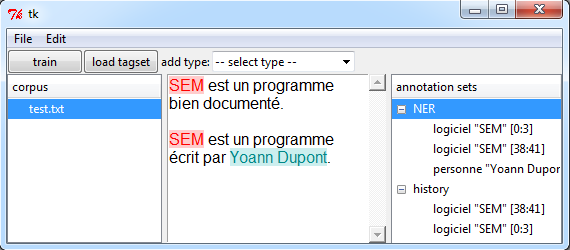
\includegraphics[scale=0.5]{fr/images/annotation_sem-05.png}
    \end{center}
    \caption{Pour annoter toutes les occurrences du document : utiliser le raccourci $<Shift+\_>$ où "\_" est le raccourci clavier pour l'étiquette. Si l'on se réfère à la figure \ref{fig:annotation_sem-04}, $<Shift+l>$ permet d'annoter toutes les occurrences de "SEM" en tant que "logiciel".}
    \label{fig:annotation_sem-05}
\end{figure}



\begin{figure}[ht!]
    \begin{center}
    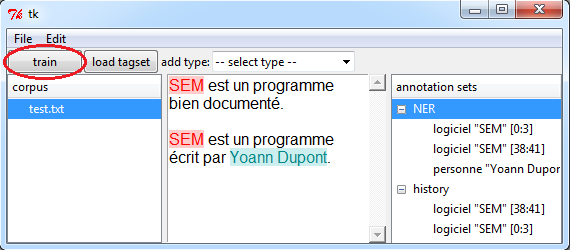
\includegraphics[scale=0.5]{fr/images/annotation_sem-06.png}
    \end{center}
    \caption{Entouré en rouge : le bouton pour entraîner SEM avec le corpus courant selon les annotations courantes. L'interface est identique à celle décrite dans la section \ref{subsubsec:train-SEM-from-annotated}.}
    \label{fig:annotation_sem-06}
\end{figure}

\end{document}
